\section{Results}
\label{sec:results}

\subsection{Subsurface habitation is a polar privilege}

Generating eight worlds at each of three site classes, at latitudes that would
actually produce them and with the solar geometry the model derives from that
latitude, gives the availability in Table~\ref{tab:sites}.

\begin{table}[htbp]
\centering
\caption{Habitat availability by site class. Medians over eight seeds.
Buildable surface is essentially unconstrained everywhere; subsurface
habitation is not.}
\label{tab:sites}
\begin{tabular}{lrrrrrr}
\toprule
site class & latitude & sun slope & buildable & ice tiles & bore sites & tube tiles \\
\midrule
polar    & $-85^\circ$ & 0.201 & 16{,}166 & 527 & 44 & 60 \\
highland & $-50^\circ$ & 0.489 & 16{,}135 & 383 &  2 &  0 \\
mare     & $-5^\circ$  & 0.859 & 16{,}297 &   2 &  0 &  0 \\
\bottomrule
\end{tabular}
\end{table}

The result is stark, and it was not designed in: it falls out of the
illumination coupling. At an equatorial mare site the shadow budget is so small
that the model places a median of two ice tiles on the entire map, no site
qualifies for a bore, and no rille --- and therefore no tube --- is generated at
all. Such a colony has exactly one way to house anyone: build on the surface.

The highland case is subtler and more interesting. Highland sites carry
substantial ice (383 tiles) but a median of only \emph{two} legal bore sites,
because that ice lies on slopes and a bore needs a level pad. Resource
abundance and resource \emph{accessibility} come apart, which is the sort of
distinction a whole-settlement model surfaces and a component model does not.

\begin{figure}[htbp]
\centering
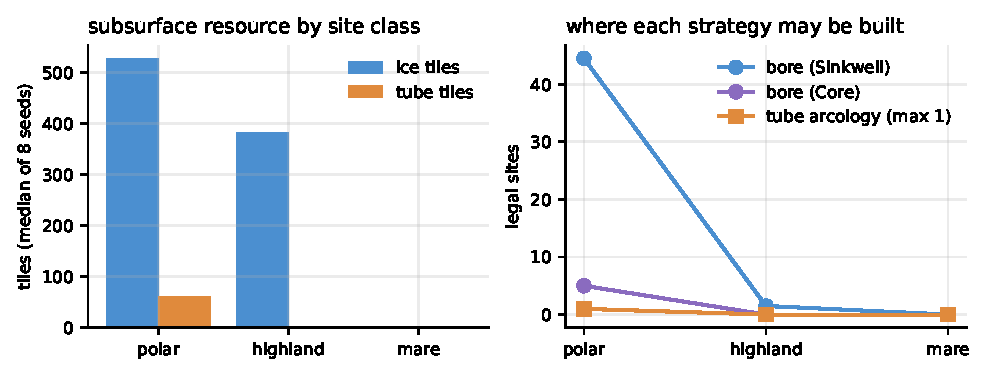
\includegraphics[width=\textwidth]{figures/site-availability.pdf}
\caption{Subsurface resource and legal sites by class. Ice is present at
highland sites but largely unusable; tubes exist only at polar sites.}
\label{fig:sites}
\end{figure}

\subsection{Arcologies buy land, not money}

Costing the three strategies on a common basis (Table~\ref{tab:econ},
Figure~\ref{fig:econ}) gives the paper's central result, and it inverts the
intuition that drove the model's design.

\begin{table}[htbp]
\centering
\caption{Habitat economics. Surface figures are for one high-density
habitation tile at its final stage. Tube figures are the median over eight
generated polar worlds; its range is $861$ to $2{,}520$ residents depending on
the tube the map produced.}
\label{tab:econ}
\begin{tabular}{lrrrr}
\toprule
strategy & residents & credits/resident & residents/kW & residents/surface tile \\
\midrule
surface tile      &    62 &   \textbf{2.4} & 31.0 &     62 \\
Sinkwell (bored)  & 1{,}100 &  58.2 & 32.4 &    122 \\
Cistern (bored)   &   480 & 170.8 & 12.0 &     53 \\
Foundry (bored)   &   405 & 182.7 &  7.8 &     45 \\
Core (bored)      & 2{,}450 & 100.0 & 25.5 &     98 \\
Tube arcology     & 2{,}295 &  41.8 & \textbf{52.2} & \textbf{2{,}295} \\
\bottomrule
\end{tabular}
\end{table}

Surface construction is between 17 and 76 times cheaper per resident than any
arcology. Whatever the case for going underground is in this model, it is not
capital efficiency.

What arcologies buy is \emph{surface area}. A tube arcology houses 2{,}295
residents while occupying a single surface tile, against 62 for the best the
surface can do --- a factor of 37. Bored arcologies achieve 45 to 122 residents
per occupied tile once their required pads are counted against them. Since the
binding constraint on a surface settlement is the ground within reach of three
utility networks, this is the currency that matters, and it is the one in which
subsurface habitation wins decisively.

The lava tube is the best deal available on every axis --- cheapest arcology
per resident, most efficient per kilowatt, and by far the most compact --- with
two compensating constraints. You get one, and its size is set by the map: the
same structure returns 861 residents on a poor tube and 2{,}520 on a generous
one, a spread of 2.9$\times$ that no decision by the player can influence. And
it returns no atmosphere, so its residents draw on pressurisation the colony
must produce elsewhere.

\begin{figure}[htbp]
\centering
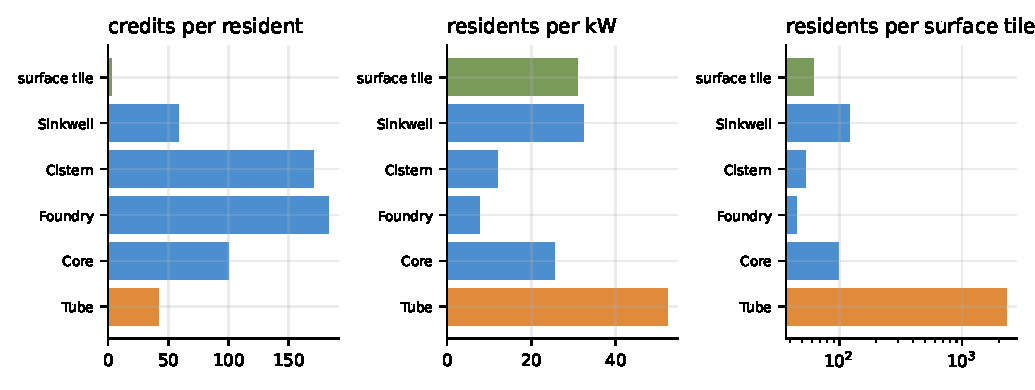
\includegraphics[width=\textwidth]{figures/habitat-economics.pdf}
\caption{The three strategies on a common basis. Surface construction wins
decisively on cost per resident; subsurface habitation wins by a larger margin
on residents per surface tile (note the logarithmic axis).}
\label{fig:econ}
\end{figure}
